\section{Introduction}

A very simple description of the Finite Elements method is given here. It might require
further development, but a list of reference works is given if more details
are needed. In particular, we recommend the book by Ern \& Guermond \cite{Ern2004}.

%The finite element method is based on two ideas: an interpolation
%method and a variational method known as \textquotedblleft weighted
%residuals\textquotedblright. Each of these methods has a similar aim: to pass
%from a continuous problem to a discrete problem. If a function $u$ is defined
%by the equation $L(u)=0$ on a continuous domain $\Omega$, the interpolation
%method will provide an approximate function of$\ u$ constructed from a finite
%number of real numbers. The variational method will replace the continuous
%equation $L(u)=0$, valid at every point of $\Omega$, by a finite number of
%equations. In short, interpolation discretizes the unknown and the variational
%principle discretizes the equation. This should be specified in a strict
%mathematical framework, which (sometimes) helps to show the existence and
%uniqueness of the solution. Unfortunately, in free surface fluid mechanics,
%these demonstrations only exist in simple cases.

The domain of computation $\Omega$ is an open and bounded domain in $\mathbb{R}^{N}$,
$\mathbb{R}$ being the set of real numbers.
$N$ is the space dimension, equal to 3 in TELEMAC-3D.
$\Gamma$ is the boundary, regular (a normal vector can be defined on it),
of $\Omega$. At the continuum level, physical quantities (pressure,
temperature, components of the velocity vector, etc.) are functions of
$\Omega$ in $\mathbb{R}$. Moreover, we require that these functions are square integrable and
$L^{2}(\Omega)$ denotes the set of square integrable functions. A dot product
can be defined on this set as:%

\begin{equation}
(u,v)_{0}=\int_{\Omega}uv~d\Omega
\end{equation}


A subset of $L^{2}(\Omega)$ is composed of functions whose derivatives along
the $N$ directions of space are also square integrable. This guarantees that a
function gradient would also be square integrable. This subset is denoted
$H^{1}(\Omega)$. A new dot product is defined in $H^{1}(\Omega)$ as:%

\begin{equation}
(u,v)_{1}=\int_{\Omega}uv+\overrightarrow{grad}(u)\cdot\overrightarrow{grad}%
(v)~d\Omega
\end{equation}


The spaces $L^{2}(\Omega)$ and $H^{1}(\Omega)$ with their dot product are
called Hilbert%
\index{Hilbert space}
spaces. Hilbert spaces are very similar to the Euclidean vector spaces. On
both of them, and with the help of the dot product, we can define:
\begin{itemize}
\item a norm:%
  \begin{equation}
    \left\|  u\right\|  =\sqrt{(u,u)}%
  \end{equation}
\item a distance:%
  \begin{equation}
    d(u,v)=\left\|  u-v\right\|
  \end{equation}
\item and an angle:%
  \begin{equation}
    \cos(\alpha)=\frac{(u,v)}{\left\Vert u\right\Vert \left\Vert v\right\Vert }%
  \end{equation}
\end{itemize}
but their dimension is infinite. $H^{1}(\Omega)$ has been described with
derivatives of the first order. $H^{k}(\Omega)$ can be described in the same
way, with derivatives of the $k$th order, like the set of functions whose
derivatives up to $k$th order are all square integrable. The $H^{k}(\Omega)$
spaces are known as Sobolev%
\index{Sobolev space}
spaces.

As for the equations being worked out, only linear equations with partial
derivatives are considered (fluid mechanics equations are generally
non-linear, but the resolution methods used for solving them will generally be
written in a linear form). Here are some of the linear equations that we shall
come across later:

Helmholtz equation:%
\index{Helmholtz equation}%
%

\begin{equation}
\frac{\partial^{2}u}{\partial x^{2}}+\frac{\partial^{2}u}{\partial y^{2}%
}+\lambda u=0
\end{equation}


Poisson equation:%
\index{Poisson equation}%
%

\begin{equation}
\frac{\partial^{2}u}{\partial x^{2}}+\frac{\partial^{2}u}{\partial y^{2}}=f
\end{equation}


In this chapter, we consider that our equation is in the form:%

\begin{equation}
L(u)=f
\end{equation}


Interpolation and the variational method will now be described more precisely.


\section{Interpolation in finite elements}

The general idea is to replace an unknown function $u$, which belongs to an
infinite dimensional space, by an approximation $u_{h}$ defined on a finite
dimensional space $N$. This is an approximation and we cannot always ensure
that $L(u_{h})=f$. We simply try to minimize $L(u_{h})-f$ and this will be the
goal of the variational method.

In finite elements, a function $u$ is represented by $n$ real numbers which
are the exact values of $u$ at special points of the domain known as degrees
of freedom. For the other points, an interpolation is sufficient. To define a
unique interpolation function, e.g. a polynomial one, with exact values of $u$
for the $n$ degrees of freedom would be very complex, or would lead at least
to a high-order function. So, finite elements give up the univocal nature of
the interpolation function and choose a locally simple interpolation function
(e.g. constant, linear, quadratic). A tessellation of space into segments,
triangles, quadrilaterals, tetrahedra, prisms, etc., is executed. The degrees
of freedom are assigned to these elements, on the vertices, at the centre of
gravity, in the middle of the sides, etc., for example. Thus, each element is
described both by the coordinates of its geometric nodes and by those of its
interpolation nodes. This is followed by a simple definition of interpolation
within each element. For example, in one dimension, taking the vertices of
segments as degrees of freedom, a linear interpolation will be chosen. The
function $u_{h}$ approximating $u$ can then be written as:%

\begin{equation}
u_{h}=\sum\limits_{i=1}^{n}u_{i}\Psi_{i}%
\end{equation}
where $\Psi_{i}$ is a basis function defined differently, but in a linear
manner, on each segment ending at the point $i$. Outside these segments,
$\Psi_{i}$ is zero. Figure \ref{base en 1D} shows this basis function in one
dimension, on a non-regular mesh. The value of $\Psi_{i}$ is 1 at point i, and
0 on all the other degrees of freedom.%

\begin{figure}[H]%
\centering
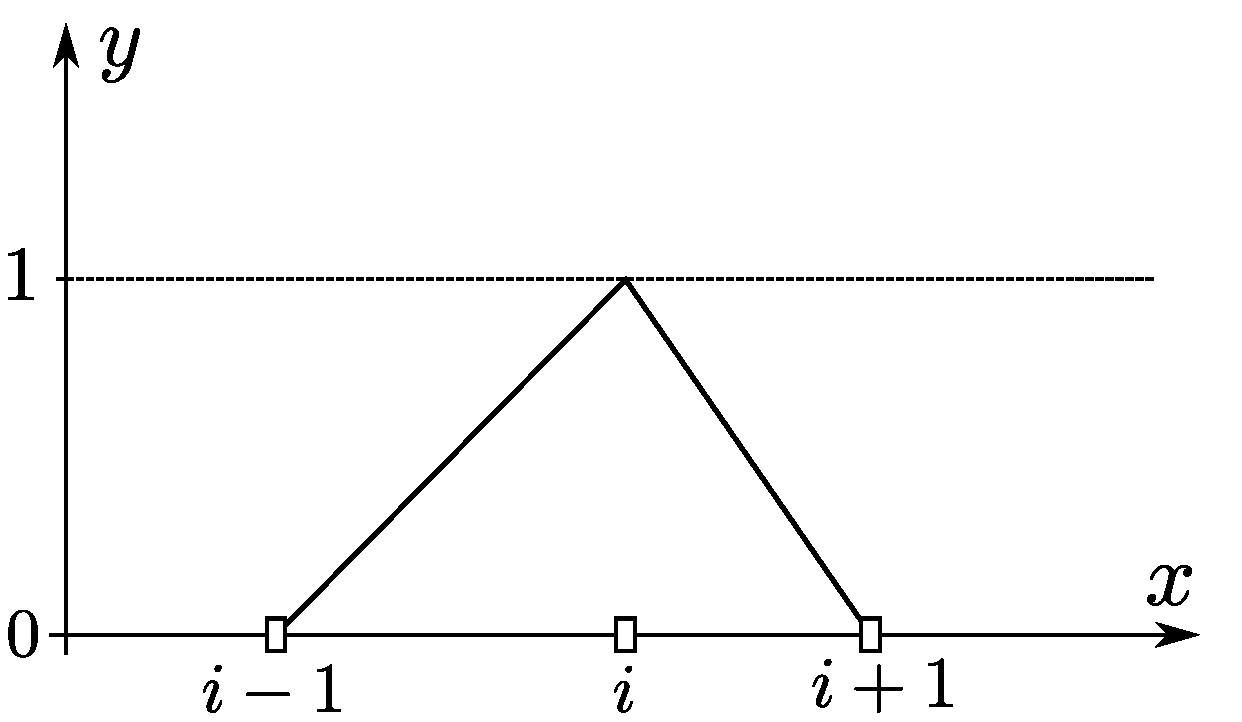
\includegraphics[scale=0.4]
{graphics/linear_basis_1D.pdf}
\caption{Shape of a linear basis in one dimension.}%
\label{base en 1D}%
\end{figure}


The property $\sum\nolimits_{i=1}^{n}\Psi_{i}=1$ is very important and will be
the key to several demonstrations. In two dimensions, with triangles and a
linear interpolation, each basis $\Psi_{i}(x,y)$ will be written as $ax+by+c$,
$a$, $b$ and $c$ depending on the triangle, so as to obtain the value 1 at
point $i$ and 0 at the other ones. Figure \ref{emprise base} shows the extent
and the nodal values of a linear basis on a finite element mesh.%

\begin{figure}[H]%
\centering
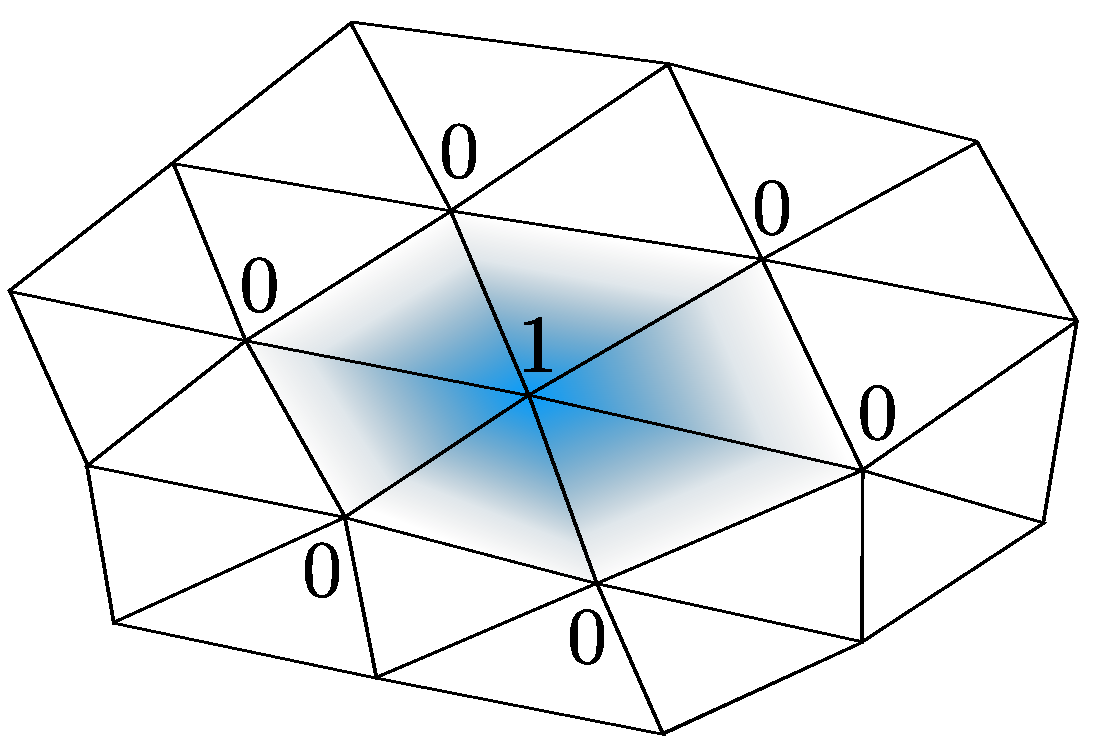
\includegraphics[scale=0.4]
{graphics/linear_basis_2D.pdf}%
\caption{Extent of a basis function on a triangular mesh. The blue color represents higher values of the basis function.}%
\label{emprise base}%
\end{figure}

These basis functions are sometimes called \textquotedblleft shape
functions\textquotedblright. With a linear interpolation, a linear function
$u$ will be represented exactly. It is said to be in the approximation space.
The interpolation can also be quadratic, or of any other order which enables
representation of the function on the degrees of freedom but also some of its derivatives.
Sometimes, and it is so for quadrilaterals, the element is too complex to get
a simple definition of the interpolation. So, we go back to a more regular
reference element (a square in the case of a quadrilateral) in a
\textquotedblleft reference\textquotedblright\ space and define a geometric
transformation between the two spaces. Interpolation is simple only in the
reference space, except in the case of simplicial elements: segments,
triangles and tetrahedra with linear interpolation. The description of
different finite elements and the use of a reference space for building finite
element matrices are explained in Reference \cite{hervouet007}. A precise
description of a large number of other elements can also be found in reference
\cite{dhatt81}.\\

%\subsection{The finite elements used in TELEMAC-3D}
In TELEMAC-3D, Lagarange finite elements are used: P1 bases on prismatic
3D elements. The bases we use can be decomposed into the poduct of
2D basis with vertical bases:
\begin{equation}
\Psi=\Psi^H\Psi^V
\end{equation}
with:
\begin{equation}
\dsum_{i=1}^{n}\Psi_i=1~,~~\dsum_{i=1}^{npoin2}\Psi_i^H=1~,~~\dsum_{i=1}^{nplan}\Psi_i^V=1
\end{equation}
where $npoin2$ is the number of points of the 2D mesh, $nplan$ is the number of
points along the vertical, $\Psi^H$ is represented in the figure \ref{emprise base} and $\Psi^V$ is
a 1-D P1 basis along $z$, as represented in the figure \ref{base en 1D}, but defined on the quadrangles composing the lateral faces of the prisms.
In order to simplify the computations of the matrices stemming from the Finite Eelements formulations, 
they are calculated in reference elements and with reference bases. 
Each element of the real mesh is transformed into a reference element, and the elementary
contributions are computed in each element in a decoupled way. In TELEMAC-3D, the
Edge-by-Edge technique is applied and there is no global matrix assembly. 
%The diagonal and extra-diagonal terms of the matrices are stored separately 
%and vectorised procedures for performing algebraic operations are provided.
The reference element used in TELEMAC-3D is shown in the figure \ref{fig:reference_element}. 

\begin{figure}
\begin{center}
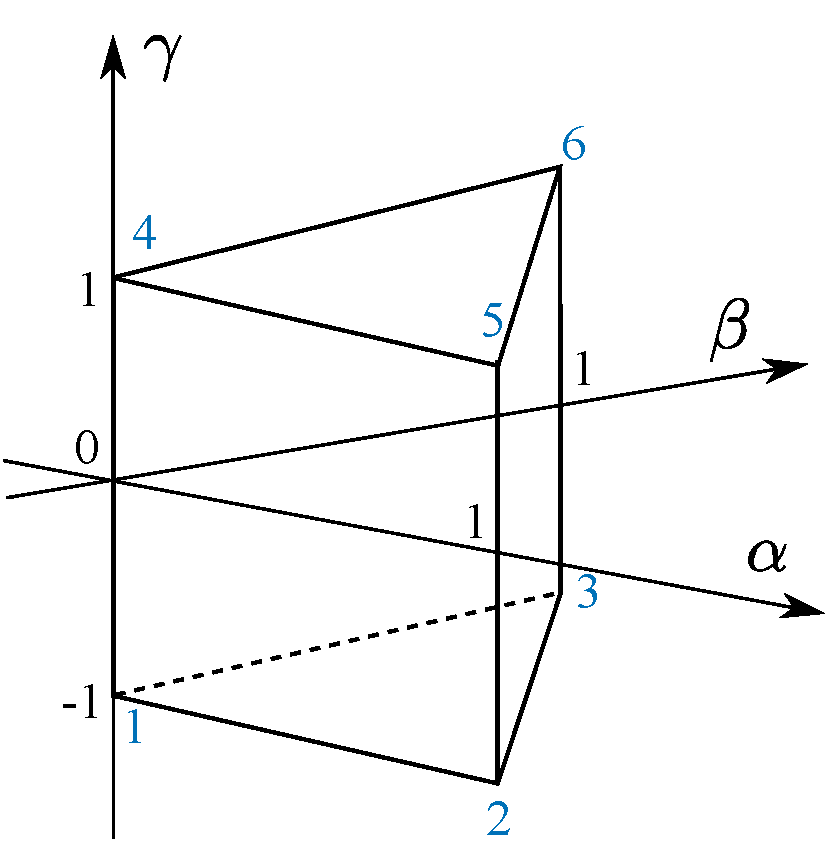
\includegraphics[scale=0.5]{./graphics/reference_element.pdf}
\end{center}
\caption{Sketch of the reference element used in TELEMAC-3D. The nodes indices
are indicated in blue whereas the coordinates in the $(\alpha, \beta, \gamma)$
system are indicated in black.}
\label{fig:reference_element}
\end{figure}

The basis functions $\Phi_i$ corresponding to the 6 nodes of the reference element read:
\begin{equation}
\begin{array}{ll}
\Phi_1 = (1-\alpha-\beta)(1-\gamma)/2 \hspace{0.5cm}& \Phi_4 = (1 - \alpha - \beta)(1 + \gamma)/2 \medskip \\
\Phi_2 = \alpha(1 - \gamma)/2 &\Phi_5 = \alpha(1 + \gamma)/2 \medskip \\
\Phi_3 = \beta(1 - \gamma)/2 &\Phi_6 = \beta(1 + \gamma)/2
\end{array}
\end{equation}

The basis functions $\Psi_i$ in the real mesh are obtained by an 
iso-parametric transformation of $\Phi_i$. The nodes of the prismatic elements 
in the real mesh have coordinates $(x_i, y_i, z_i)$. 
The coordinates of a point $P(x, y, z)$ within an element of the real mesh
are related to the coordinates in the reference element by:
\begin{equation}
x=\sum_{i=1}^6x_i\Phi_i(\alpha,\beta,\gamma)~,~~~y=\sum_{i=1}^6y_i\Phi_i(\alpha,\beta,\gamma)~,~~~z=\sum_{i=1}^6z_i\Phi_i(\alpha,\beta,\gamma)
\label{eq:xprism}
\end{equation}
Since the lateral faces of the prisms are vertical, some coordinates coincide: 
$x_1=x_4$, $y_1=y_4$, $x_2=x_5$, $y_2=y_5$, $x_3=x_6$, $y_3=y_6$, so that the
relations \eqref{eq:xprism} are simplified into:
\begin{equation}
\begin{array}{l}
x = (1-\alpha-\beta)x_1+\alpha x_2+\beta x_3 \medskip\\
y = (1-\alpha-\beta)y_1+\alpha y_2+\beta y_3 \medskip\\
z = \dfrac{1}{2}\left[(1-\alpha-\beta)z_1+\alpha z_2+\beta z_3\right](1-\gamma)+
 \dfrac{1}{2}\left[(1-\alpha-\beta)z_4+\alpha z_5+\beta z_6\right](1+\gamma)
\end{array}
\end{equation}
The Jacobian of this transformation, denoted by $|\vec{J}|$, reads:
\begin{equation}
\begin{array}{ll}
|\vec{J}|& =\dfrac{1}{2}\left[(x_2-x_1)(y_3-y_1)+(x_1-x_3)(y_2-y_1)\right]\medskip \\
& \left[(1-\alpha-\beta)z_4+\alpha z_5+\beta z_6-(1-\alpha-\beta)z_1-\alpha z_2
-\beta z_3\right]
\end{array}
\label{eq:jacobian}
\end{equation}
Let $F$ be the transformation that from $(\alpha, \beta, \gamma)$ 
yields $(x,y,z)$. The bases in the real mesh $\Psi_i$ are obtained 
from the bases in the reference element through:
\begin{equation}
\Psi_i(x,y,z)=\Phi_i(F^{-1}(x,y,z))
\label{eq:transfF}
\end{equation}

In some parts of the algorithm a two-dimensional approach is needed, 
as \textit{e.g.} in the free-surface step or for the computation of the 
friction in the diffusion step. In the case of the 2-D integrals, triangular 
elements with linear interpolation are used. For vertical lateral boundaries, 
quadrilaterals with linear interpolation are used. 
The reference elements are: a triangle with nodes at $(0, 0)$, $(0, 1)$, $(1, 0)$ and a square with nodes $(-1,-1)$, $(1,-1)$, $(1, 1)$, $(-1, 1)$, as 
represented in the figure \ref{fig:reference_elements_2D}.
The linear interpolation functions for the triangle are:
\begin{equation}
\Phi_1 = (1 - \xi - \lambda)
\Phi_2 = \xi
\Phi_3 = \lambda
\end{equation}
and for the quadrilaterals:
\begin{equation}
\Phi_1 = (1 - \xi - \lambda + \xi\lambda)/4
\Phi_2 = (1 + \xi - \lambda - \xi\lambda/4
\Phi_3 = (1 + \xi + \lambda + \xi\lambda)/4
\Phi_4 = (1 - \xi + \lambda - \xi\lambda)/4
\end{equation}
\begin{figure}
\begin{center}
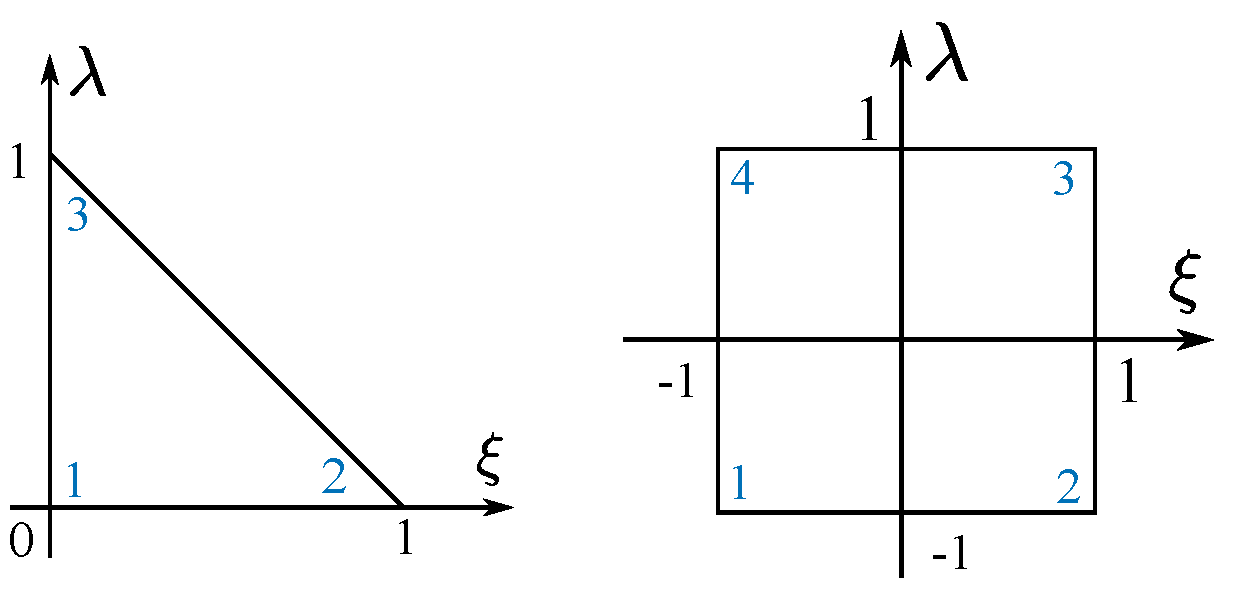
\includegraphics[scale=0.5]{./graphics/reference_elements_2D.pdf}
\end{center}
\caption{Sketch of the 2D reference elements used in TELEMAC-3D. 
The nodes indices are indicated in blue whereas the coordinates in the
local referential of each element are indicated in black.}
\label{fig:reference_elements_2D}
\end{figure}

\section{Variational principle for boundary value problems%
\index{variational formulation}%
}

Having restricted our function $u$ to a representation $u_{h}$, based on a
discrete number of unknowns $u_{i}$, we now wish to minimize $L(u_{h})-f$. The
variational method states that the dot product
$\int_{\Omega}(L(u_{h})-f)\varphi_{i}~d\Omega$
is zero for some functions $\varphi_{i}$ called test
functions\index{test function}.
The choice of these functions defines the variants of the finite element
method. The most classical technique, the Galerkin technique, consists in
choosing test functions equal to the basis functions: $\varphi_{i}=\Psi_{i}$.
In this case, if $u_{h}$ is decomposed as $\sum\nolimits_{i=1}^{n}u_{i}%
\Psi_{i}$, the variational method will clearly lead to a linear system of
unknowns $u_{i}$.

Moreover, to each linear operator $L$ is associated a bilinear form $a$ such as:%

\begin{equation}
a(u,v)=\int_{\Omega}(L(u)-f)\,v\,d\Omega
\end{equation}


The finite element theory aims at determining the conditions on $L$ and on $a
$ for which the problem would have a unique solution. An important condition
is that, for every non-zero function $u$, there exists a real $\alpha$
positive, such that $\left\Vert L(u)\right\Vert \geq\alpha\left\Vert
u\right\Vert $. If the norm $L$ is defined by:
\[
\left\Vert L\right\Vert =\sup_{u\neq0}\left(  \frac{\left\Vert L(u)\right\Vert
}{\left\Vert u\right\Vert }\right)
\]
this condition signifies that $L$ should have a strictly positive norm.
Otherwise, if a non-zero function $u_{p}$ verifies $L(u_{p})=0$, the solution
will not be unique because if $u$ is a solution of the equation $L(u)=f$,
$\ u+u_{p}$ will also be one. Within the variational method frame, the
condition is written as:%

\begin{equation}
\inf_{u\neq0}\left(  \sup_{v\neq0}\left(  \frac{a(u,v)}{\left\Vert
u\right\Vert \left\Vert v\right\Vert }\right)  \right)  \geq\alpha
\end{equation}


This is known as the \textquotedblleft inf--sup condition\textquotedblright%
\index{inf--sup condition}%
. It prevents the occurrence of parasitic solutions which could arise from the
bilinear form. For example, for a one-dimensional domain with regularly spaced
degrees of freedom, if $L$ is the gradient operator, and if the basis
functions $\Psi_{i}$ are linear and equal to the test functions $\varphi_{i}$,
a function $u$ whose values at the nodes are a succession of 1 and $-$1 (see
Figure \ref{parasite}) would lead to $\int\nolimits_{\Omega}L(u)\varphi
_{i}d\Omega=0$ for every test function $\varphi_{i}$ and the inf--sup
condition would not be verified.%

%TCIMACRO{\FRAME{ftbpFU}{11.4246cm}{4.0835cm}{0pt}{\Qcb{an invisible function
%for the gradient operator}}{\Qlb{parasite}}{Figure}%
%{\special{ language "Scientific Word";  type "GRAPHIC";
%maintain-aspect-ratio TRUE;  display "USEDEF";  valid_file "T";
%width 11.4246cm;  height 4.0835cm;  depth 0pt;  original-width 6.3866in;
%original-height 2.2563in;  cropleft "0";  croptop "1";  cropright "1";
%cropbottom "0";  tempfilename 'NG0IDC04.wmf';tempfile-properties "XPR";}} }%
%BeginExpansion
\begin{figure}[H]%
\centering
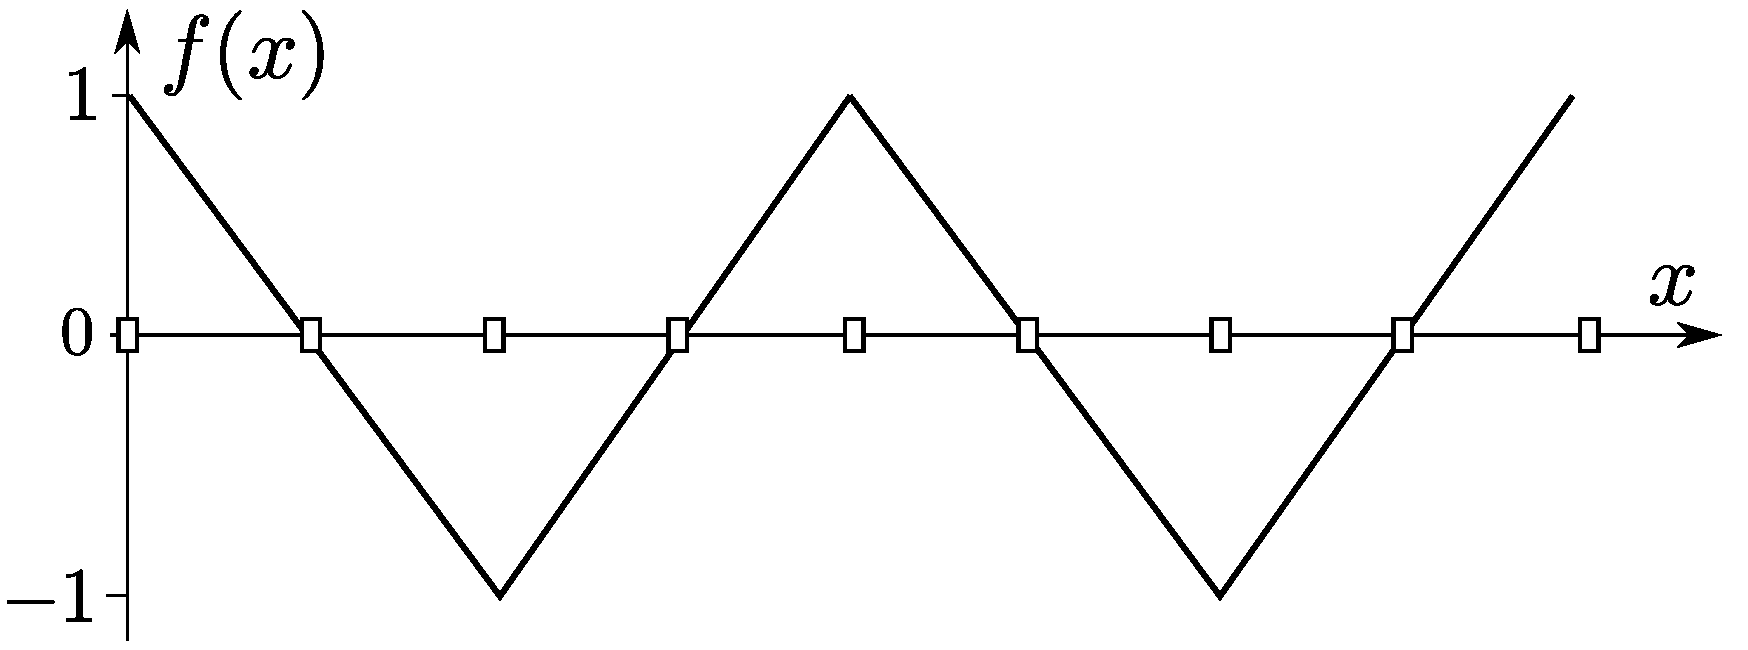
\includegraphics[scale=0.4]
{graphics/invisible_gradient.pdf}%
\caption{An example of invisible function for the gradient operator.}%
\label{parasite}%
\end{figure}
%EndExpansion


This situation arises when the boundary conditions are not considered, but it
can take place also far from the boundaries of a calculation domain. The
bilinear forms resulting from the variational formulations of the
Navier--Stokes equations do not always satisfy the inf--sup condition. A
well-known condition for internal flows of incompressible fluids consists in
choosing different elements to represent pressure and velocity: for example, a
quadratic velocity and a linear pressure.
%In principle, this choice is not
%mandatory for compressible fluids and, by extension, for the Saint-Venant
%equations. However, the choice of different elements for velocity and water
%depth gives more regular results. This is exemplified in Plate 5, where a tide
%is simulated on a quarter-circle beach with a quadratic bottom elevation.
%Advection and all dissipative terms are removed from equations. It is clear
%that in this academic situation spurious oscillations occur with a linear
%discretization, but they disappear if the velocity is treated with a
%quasi-bubble discretization (see \cite{atkinson01}\ for more details).
Another solution, efficient with regular mesh and the finite difference method, is to
have two different and staggered meshes for pressure and velocity. Finally,
for elliptic equations, we can use a discretization of the Laplacian, known as
\textquotedblleft non-compatible\textquotedblright, for which the Laplacian is
not, at the discrete level, equal to the divergence of the gradient.
%The result of this method is detailed in Section \ref{equation d'onde}, where the
%Saint-Venant equations are written in the form of a wave equation.

A more thorough examination of these questions, especially for the
Navier--Stokes equations, can be found in references \cite{ciarlet78} and
\cite{raviart86}, and in the more recent work by Pironneau \cite{pironneau88}
on the methods of finite elements for fluids.

%\subsection{Discretisation of the Navier--Stokes equations in a fixed mesh}


%In TELEMAC-3D a fractional-steps method is used for the time discretisation.
%An important aspect of the algorithm is that the horizontal and vertical velocities are
%not treated the same way. Moreover, there are two definitions of the velocity field
%in the algorithm: the one calculated on the basis of the continuity equation so as to ensure
%mass conservation and the one calculated on the basis of the momentum equation. Later on,
%we refer to them as the conservative velocity and the momentum velocity fields.
%The algorithm then consists of several steps, namely:
%\begin{itemize}
%\item an advection step for the momentum horizontal velocities, using the conservative velocity for the advection;
%\item an advection-diffusion step for the momentum vertical velocity, using the conservative velocity field for the advection and the momentum velocity for the diffusion;
%\item a hydrostatic step, which consists of computing the new depth
%together with the conservative horizontal velocities and then deducing the conservative vertical velocity;
%\item a pressure step for computing the non-hydrostatic pressure and calculating the momentum velocity field;
%\item a final advection-diffusion step for tracers, using the conservative velocity field for the advection.
%\end{itemize}
%
%%Each of these steps will be resolved in detail one after the other. Prior to this,
%%however, discretization in space and building up the mesh have to be specified.
%The sections below describe the hydrostatic step, the pressure step and the tracers advection-diffusion step.
%
%\section{Hydrostatic step}
%
%\subsection{Wave equation}
%\begin{equation}
%  \begin{array}{l}
%    \dfrac{\vec{u}_{2D}^{\textcolor{EdfBlue}{A}}-\vec{u}_{2D}^n}{\delta t}
%    + \left(\left(\vec{u}^{\textcolor{EdfBlue}{A}}-\vec{c}\right)\cdot\Grad\right)\vec{u}_{2D}^{\textcolor{EdfBlue}{A}}=0 \medskip \\
%    \dfrac{w^{\textcolor{EdfOrange}{D}}-w^n}{\delta t}+
%    \left(\left(\vec{u}^{\textcolor{EdfOrange}{D}}-\vec{c}\right)\cdot\Grad\right)w^{\textcolor{EdfOrange}{D}}=
%    -g+\Div(\nu\vec{S}\cdot\vec{e}_z)
%  \end{array}
%\end{equation}
%
%\begin{equation}
%  \begin{array}{l}
%    \dfrac{\eta^{n+1}-\eta^{n}}{\delta t}
%    + \nabla_{2D}\cdot \displaystyle{\int_b^\eta\vec{u}_{2D}^{\textcolor{EdfOrange}{D}}}=0 \medskip \\
%    \dfrac{\vec{u}_{2D}^{\textcolor{EdfOrange}{D}}-\vec{u}_{2D}^{\textcolor{EdfBlue}{A}}}{\delta t}=-g\Grad_{2D}\eta^{n+1}
%    +\Div\left(\nu(\vec{S}\cdot\vec{e}_x+\vec{S}\cdot\vec{e}_y)\right)
%  \end{array}
%\end{equation}
%
%\subsection{Vertical velocities}
%
%%The time-discretisation is done following the sequence below:
%
%%\begin{align}
%%&\frac{\tilde{\vec{U}}_{2D}^{n+1}-\vec{U}_{2D}^{n}}{\Delta t} = - \vec{U}^n\cdot\Grad \vec{U}_{2D}^n + \vec{F}_{2D}^{visc^{n+1}} + \tilde{\vec{F}}_{2D}^{n+1}
%%\notag\\
%%&\frac{\eta^{n+1}-\eta^{n}}{\Delta t} = - \DivD\left(\int_b^\eta\tilde{\vec{U}}_{2D}^ndz\right) + F_b^n
%%\notag\\
%%&\frac{\tilde{W}^{n+1}-W^{n}}{\Delta t} = - \vec{U}^n\cdot\Grad W^n + F_z^{visc^{n+1}} + F_z^{n+1}
%%\notag\\
%%&\Div \left(\frac{1}{\rho}\Grad p_d^{n+1}\right) = \frac{1}{\Delta t}\Div\tilde{\vec{U}}^{n+1}
%%\notag\\
%%&\frac{\vec{U}^{n+1}-\tilde{\vec{U}}^{n+1}}{\Delta t} = - \frac{1}{\rho}\Grad p_d^{n+1}
%%\label{eq:NS_FS_timestepping}
%%\end{align}
%%
%%\commentAL{La convection des vitesses est faite
%%avec les vitesses du pas de temps précédent
%%et la convection des traceurs est faite
%%avec $\Delta z W^*$ afin de conserver la masse de traceur.}
%
%\section{Pressure step}
%\begin{equation}
%  \begin{array}{l}
%    \Lap p_d^{n+1} = \dfrac{\rho}{\delta t}\Div\vec{u}^{\textcolor{EdfOrange}{D}} \medskip \\
%    \dfrac{\vec{u}^{n+1}-\vec{u}^{\textcolor{EdfOrange}{D}}}{\delta t} = -\dfrac{1}{\rho}\Grad p_d^{n+1}
%  \end{array}
%\end{equation}
%
%\section{Tracers advection-diffusion}
